\appendix

\section{ODEs on the moments} \label{calc}

\subsection{One dimensional case}
We start from the diffusion model for the frequency spectrum evolution in a single population (1 dimension):
\begin{equation}
\begin{split}
\p{\phi(x,t)}{t}\simeq &\frac{1}{4 N} \pd{}{x} x(1-x) \phi(x,t) \\&-s \p{}{x} \left(h+(1-2h)x \right)x (1-x) \phi(x,t) \\&+ 2 N u \delta(x-\frac{1}{2 N}).
\end{split}
\label{eq:diff}
\end{equation}

The first term of the right hand side is a diffusion term modeling the effect of genetic drift, the second one is a transport term that accounts for the selection. Finally, the source term $ 2 N u \delta(x-\frac{1}{2 N})$ reproduces the mutations process.\\
We are interested in the moment-like statistics $$ \Phi_n(i) = \int_0^1 {n\choose i}  x^i (1-x)^{n-i} \phi dx,$$ and we would like to find evolution laws for these quantities using the diffusion equation above.\\
So we can write the time derivative of  $\Phi_n(i)$ : 
$$\dot \Phi_n(i) = \int_0^1 w_i \dot \phi dx,$$
with $w_i=  {n\choose i}  x^i (1-x)^{n-i}$.\\
The mutation term is modeled differently and separately. In the continuous model, it is assumed that the mutations are injected at frequency $x=\frac{1}{2 N}$. That amounts to saying that each mutation appears in a single individual at the time. In our discrete approach, we inject the mutations as a new singleton so the mutation term writes $2 N u \delta_{i=1}$. Using this and replacing $\dot \phi$ by the approximation given by Eq.\eqref{eq:diff} we have:
\begin{equation}
\begin{split}
	\dot \Phi_n(i) &= 2 n u \delta_{i=1} + \frac{1}{4 N} \int_0^1 w_i \pd{}{x}\left( x(1-x) \phi(x,t)\right)dx \\
			     & - s\int_0^1w_i \p{}{x}\left( \left(h+(1-2h)x \right)x (1-x) \phi(x,t)\right)dx.
\end{split}
\label{eq:diff2}
\end{equation}

\paragraph{drift term:}
We want to rewrite the drift term of equation \eqref{eq:diff2} in terms of the moments $\Phi_n(i)$. To do that, we can integrate by parts:
\begin{equation*}
\begin{split}
	\frac{1}{4 N}\int_0^1 w_i \pd{}{x}\left( x(1-x) \phi(x,t)\right)dx &= \frac{1}{4 N}\left[w_i \p{}{x}\left( x(1-x) \phi(x,t)\right)\right]_0^1\\
			     & -\frac{1}{4 N} \int_0^1 \p{w_i}{x}\p{}{x}\left( x(1-x) \phi(x,t)\right)dx.
\end{split}
\end{equation*}
As $w_i(0)=w_i(1)=0$ we assume that the first terms is $0$. We can integrate by parts the second term:
\begin{equation*}
\begin{split}
	\frac{1}{4 N}\int_0^1 w_i \pd{}{x}\left( x(1-x) \phi(x,t)\right)dx &= -\frac{1}{4 N} \int_0^1 \p{w_i}{x}\p{}{x}\left( x(1-x) \phi(x,t)\right)dx\\
	& = -\frac{1}{4 N}\left[\p{w_i}{x} \times  x(1-x) \phi(x,t)\right]_0^1\\
	& + \frac{1}{4 N}\int_0^1\pd{w_i}{x} x(1-x) \phi(x,t)dx.
\end{split}
\end{equation*}
As we consider a finite genome, $ \phi(0,t)$ and $ \phi(1,t)$ are finite and, once again, the term in square brackets is zero. Moreover, we have:
\begin{equation*}
\begin{split}
\pd{w_i}{x} &= {n\choose i} \Big[ i\left[(i-1)x^{i-1}(i-x)^{n-i}-(n-i)x�(1-x)^{n-i-1}\right] \\
		&- (n-i)\left[ix^{i-1}(1-x)^{n-i-1} - (n-i-1)x�(1-x)^{n-i-2}\right]\Big].
\end{split}
\end{equation*}
Thus,
\begin{equation*}
\begin{split}
\text{drift term} &=\frac{1}{4 N}\int_0^1\pd{w_i}{x} x(1-x) \phi(x,t)dx\\
		&= \frac{1}{4 N}\Big[\int_0^1{n\choose i} i(i-1)x^i(i-x)^{n-i+1}\phi(x,t)dx\\
		&-\int_0^1{n\choose i}i(n-i)x^{i+1}(1-x)^{n-i}\phi(x,t)dx \\
		&-\int_0^1{n\choose i} (n-i)ix^i(1-x)^{n-i} \phi(x,t)dx \\
		&+\int_0^1{n\choose i}(n-i)(n-i-1)x^{i+1}(1-x)^{n-i-1}\phi(x,t)dx\Big].
\end{split}
\end{equation*}
Rearranging this expression, we can write it in terms of the $\Phi_n(i)$:
\begin{equation*}
\begin{split}
\text{drift term} &=\frac{1}{4 N} \left[ (i-1)(n-i+1) \Phi_n(i-1)\delta_{i\geq 2} \right.\\
		      & \left.-2i(n-i)\Phi_n(i)\delta_{1\leq i\leq n-1}  + (n-i-1)(i+1)\Phi_n(i+1)\delta_{i\leq n-2} \right]
\end{split}
\end{equation*}
\paragraph{selection term:}
Here again, we integrate by parts the selection term.
\begin{equation*}
\begin{split}
 - s\int_0^1w_i \p{}{x}\left( \left(h+(1-2h)x \right)x (1-x) \phi(x,t)\right)dx &= -s\left[ w_i \left(h+(1-2h)x \right)x (1-x) \phi(x,t)\right]_0^1\\
 	&+ s\int_0^1 \p{w_i}{x}\left(h+(1-2h)x \right)x (1-x) \phi(x,t)dx.
 \end{split}
\end{equation*}
We can again assume that the term in square brackets is zero, we rearrange the other integral term in order to write it in terms of the $\Phi_n(i)$. We finally get: 
\begin{equation*}
\begin{split}
 \text{selection term} &= \frac{sh}{n+1}\left[i(n+1-i)\Phi_{n+1}(i)-(n-i)(i+1)\Phi_{n+1}(i+1)\right] \\
		      & +\frac{s(1-2h)(i+1)}{(n+1)(n+2)}\left[i(n+1-i)\Phi_{n+2}(i+1)-(n-i)(i+2)\Phi_{n+2}(i+2)\right].
 \end{split}
\end{equation*}
\paragraph{}
Bringing these expressions together, we get a system of ordinary differential equations on the $\Phi_n(i)$:
\begin{equation}
\begin{split}
\dot \Phi_n(i)=& 2nu  \delta_{i=1} + \frac{1}{4 N} \left[ (i-1)(n-i+1) \Phi_n(i-1)\delta_{i\geq 2} \right.\\
		      & \left.-2i(n-i)\Phi_n(i)\delta_{1\leq i\leq n-1}  + (n-i-1)(i+1)\Phi_n(i+1)\delta_{i\leq n-2} \right]\\
		      &+ \frac{sh}{n+1}\left[i(n+1-i)\Phi_{n+1}(i)-(n-i)(i+1)\Phi_{n+1}(i+1)\right] \\
		      & +\frac{s(1-2h)(i+1)}{(n+1)(n+2)}\left[i(n+1-i)\Phi_{n+2}(i+1)-(n-i)(i+2)\Phi_{n+2}(i+2)\right].
\end{split}
\label{eq:syst_edo}
\end{equation}

\subsection{Extension to multiple dimensions}\label{multidimcalc}
The diffusion model can be generalized to multiple populations studies. The drift, selection and mutation terms are directly derived from the unidimensional case. We just need to add the effect of the migrations between the populations. The equation on the join frequency spectrum is:

\begin{equation}
\begin{split}
\p{\phi(\textbf{x},t)}{t}\simeq & \sum_{j=1}^p \bigg[ \frac{1}{4 N_j} \pd{}{x_j} \Big( x_j(1-x_j) \phi(\textbf{x},t)\Big) \\
					&-s_j \p{}{x_j}\Big( \left(h_j+(1-2h_j)x_j \right)x_j (1-x_j) \phi(\textbf{x},t)\Big) \\
					&-\sum_{k \neq j}m_{jk}\p{}{x_j}\Big( (x_k-x_j) \phi(\textbf{x},t)\Big)\\
					&+ 2 N_j u \delta(x_j-\frac{1}{2 N_j})\Pi_{k\neq j}\delta(x_k)\bigg].
\end{split}
\label{eq:diffnp}
\end{equation}
Now $\textbf{x}$ is a vector: $\textbf{x}=[x_1,\cdots,x_p] \in [0;1]^p$. It is the same for the parameters $\textbf{s}$ and $\textbf{h}$ and $N_j$ is the reference population size for population $j$. The term $-\sum_{j=1}^p \sum_{k \neq j}m_{jk}\p{}{x_j}\Big( (x_k-x_j) \phi(\textbf{x},t)\Big)$ accounts for the migrations where $m_{jk}$ is the migration rate from population $k$ to population $j$.\\
We are interested in the multi dimensional statistics generalizing the $\Phi{n}(i)$:
$$
\Phi_{\mathbf{n}}(\mathbf{i})= \int \prod_{j=1}^p { n_j \choose i_j} x_j^i (1-x_j)^{n_j-i_j} dx_j \phi(\mathbf{x}), 
$$
where $\mathbf{n}$ and $\mathbf{i}$ are vectors. The calculations are a bit more tedious but we can do the same as for the single population case, integrating by parts each term and writing it in terms of the $\Phi_{\mathbf{n}}(\mathbf{i})$, we get:
\begin{equation}
\begin{split}
\dot \Phi_\mathbf{n}(\mathbf{i})=& \sum_{j=1}^p \bigg[ n_j u  \delta_{i_j=1,i_k=0,k \neq i} + \frac{1}{4 N_j} \left[ (i_j-1)(n_j-i_j+1) \Phi_\mathbf{n}(\mathbf{i-e_j}) \right.\\
		      & \left.-2i_j(n_j-i_j)\Phi_\mathbf{n}(\mathbf{i}) + (n_j-i_j-1)(i_j+1)\Phi_\mathbf{n}(\mathbf{i+e_j})\right]\\
		      &+ \frac{s_jh_j}{n_j+1}\left[i_j(n_j+1-i_j)\Phi_\mathbf{n+e_j}(\mathbf{i})\right.\\
		      & \left.-(n_j-i_j)(i_j+1)\Phi_\mathbf{n+e_j}(\mathbf{i+e_j})\right] \\
		      & +\frac{s_j(1-2h_j)(i_j+1)}{(n_j+1)(n_j+2)}\left[i_j(n_j+1-i_j)\Phi_\mathbf{n+2e_j}(\mathbf{i+e_j})\right.\\
		      & \left.-(n_j-i_j)(i_j+2)\Phi_\mathbf{n+2e_j}(\mathbf{i+2e_j})\right]\\
		      & + \sum_{k\neq j}m_{jk}\Big[\frac{n_j(i_k+1)}{n_k+1}\left(\Phi_\mathbf{n+e_k-e_j}(\mathbf{i+e_k-e_j}) - \Phi_\mathbf{n+e_k-e_j}(\mathbf{i+e_k})\right)\\
		      & - i_j \Phi_\mathbf{n}(\mathbf{i}) + (i_j+1)\Phi_\mathbf{n}(\mathbf{i+e_j})\Big] \bigg].
\end{split}\label{eq:edond}
\end{equation}
Here, $\mathbf{e_j}$ is the $i_{th}$ vector of the canonical basis of $\mathbb{R}^p$ ($\mathbf{e_j}(i)=\delta_{ij}$).

\section{Jackknife approximation for moment closure}
The coupled ODEs system obtained integrating the diffusion equation involves higher order terms such as $\Phi_{n+1}$ or $\Phi_{n+2}$. Consequently it is not closed and cannot be solved as is. To tackle this, we use a Jackknife approach to approximate these terms.\\
In a few words, the Jackknife method consists here in writing the $n+1$ (or $n+2$) order term as a linear combination of current order terms:
$$
	\Phi_{n+1}(i) \simeq \sum_{k \in I_i} \alpha_k \Phi_n(k),
$$
where $I_i$ is the set of indexes we use in the approximation of $\Phi_{n+1}(i)$. The order of the Jackknife depends on the number of current order terms we use in the approximation ($i.e.$ the cardinal of $I$). The specificity of the method is that we compute the coefficients $\alpha_k$ to cancel the approximation error for $\Phi$ in a certain family of functions.\\
The higher order the Jackknife is, the more accurate the estimation can be but the more complicated the calculations are.
The choice of the family of functions for which the Jackknife is exact is limited by the order of the method. For instance if we want to use an order 2 Jackknife, it means that we just use two $n$ order terms in the approximation and our functions must be parameterized with these two terms. So we can use affine functions. With an order 3 Jackknife, we could cancel the error for quadratic functions and so on.\\
We will focus here on the order 2 Jackknife for the terms $\Phi_{n+1}(i)$ and we will use the following approximation:
$$
	\forall i \in [2;n-1], \Phi_{n+1}(i) = \alpha_i \Phi_n(i-1)+\beta_i \Phi_n(i), 
$$
$$
	\Phi_{n+1}(1) = \alpha_1 \Phi_n(1)+\beta_1 \Phi_n(2),
$$
and
$$
	\Phi_{n+1}(n) = \alpha_n \Phi_n(n-2)+\beta_n \Phi_n(n-1).
$$
The indexes $i=1$ and $i=n$ must be considered separately. We will detail the general case $i \in [2;n-1]$ in the following paragraph, the other cases can be computed similarly.\\
As we use an order 2 Jackknife, we chose to cancel the approximation error for affine functions and we compute the coefficients $\alpha_i$ and $beta_i$ to this aim. The assumption is:
$$
	\phi(x) = ax+b(1-x).
$$
And the statistics become:
$$
	\Phi_n(i)=\int_0^1{n \choose i}x_i(1-x)^{n-i}\left[ax+b(1-x)\right]dx.
$$

In this case, it can be expressed explicitly (using Mathematica), we finally get:
$$
	\Phi_n(i) = \frac{a+b+ai-bi+bn}{(n+1)(n+2)}.
$$
We look for the Jackknife coefficients $\alpha_i$ and $\beta_i$ such as the approximation error is zero:

$$
	\Phi_{n+1}(i)-\alpha_i \Phi_n(i-1)-\beta_i \Phi_n(i)=0.
$$
We then replace the $\Phi$ by their expressions:
$$
	\frac{a(1+i)+b(2-i+n)}{(n+2)(n+3)}-\alpha_i \frac{ai+b(2-i+n)}{(n+1)(n+2)}-\beta_i\frac{a(1+i)+b(1-i+n)}{(n+1)(n+2)} = 0.
$$
This equation is true whatever the coefficients $a$ and $b$ so we can use the particular values $(1,0)$ and $(0,1)$ and write the corresponding system of equations:

$$
  \left\{
      \begin{aligned}
        &\alpha_i i +\beta_i(i+1) = \frac{(i+1)(1+n)}{n+3},\\
        &\alpha_i (2-i+n) +\beta_i(1-i+n) = \frac{(2-i+n)(1+n)}{n+3}.
      \end{aligned}
    \right.
$$ 


We can compute the jackknife coefficients $\alpha_i$ and $\beta_i$ solving the previous linear system. We finally get:
$$
  \left\{
      \begin{aligned}
        &\alpha_i = \frac{(i+1)(1+n)}{(n+2)(n+3)},\\
        &\beta_i = \frac{(1+n)(2-i+n)}{(n+2)(n+3)}.
      \end{aligned}
    \right.
$$ 

\section{Numerical details}
\subsection{Bidirectional splitting}
Numerical resolution of partial differential equations in several dimensions generally involves directional splitting to drastically reduce computational time. In our case, the ordinary differential equations system we consider is comparable to a PDE, each population being seen as a direction. It seems thus justifiable to use a directional splitting to make our simulations more efficient. 

However, the migration term induces diagonal dependencies. That means, for a 2 populations case, that $\dot \Phi_{n_1,n_2}(i_1, i_2)$ depends on terms such as $\Phi_{n_1,n_2}(i_1+1, i_2+1)$ or $\Phi_{n_1,n_2}(i_1+1, i_2-1)$. This makes it impossible to properly split the numerical resolution and consider separately each dimension. 

To overcome this problem, we split the resolution by pairs of dimensions or populations so we can deal with the diagonal terms (see Fig.\ref{fig:split2d} for an illustration on a 3 dimensional case). 
 \begin{figure}[h]
\centering
	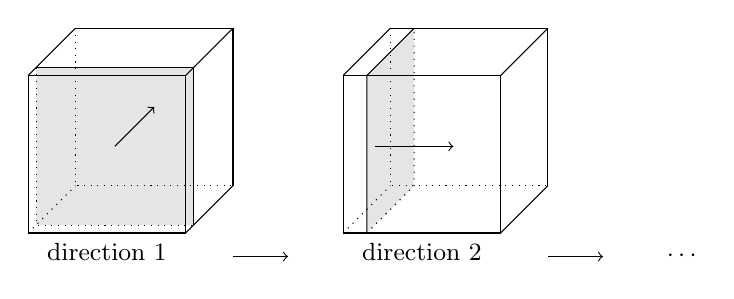
\begin{tikzpicture}
	\fill[color=gray!20] (0,0) -- (2,0) -- (2,2) -- (0,2) -- cycle;
	\draw [dotted] (0,2)  -- (0,0) -- (2,0) ;
	\draw (2,0) -- (2,2) -- (0,2) ;
	\draw (-0.1,-0.1) -- (1.9,-0.1) -- (1.9,1.9) -- (-0.1,1.9) -- cycle;
	\draw [dotted] (0.5,2.5) -- (0.5,0.5) -- (2.5,0.5);
	\draw (2.5,0.5) -- (2.5,2.5) -- (0.5,2.5);
	\draw (1.9,1.9) -- (2.5,2.5);
	\draw (-0.1,1.9)--(0.5,2.5);
	\draw (1.9,-0.1)--(2.5,0.5);
	\draw[dotted] (-0.1,-0.1)--(0.5,0.5);
	\draw[->] (1,1) -- (1.5,1.5);
	\draw(0.9,-0.1) node[below]{\small direction 1} ;
	
	\fill[color=gray!20] (4.2,-0.1) -- (4.2,1.9) -- (4.8,2.5) -- (4.8,0.5) -- cycle;
	\draw (4.2,-0.1) -- (4.2,1.9) -- (4.8,2.5);
	\draw[dotted] (4.2,-0.1) -- (4.8,0.5) -- (4.8,2.5);
	\draw (3.9,-0.1) -- (5.9,-0.1) -- (5.9,1.9) -- (3.9,1.9) -- cycle;
	\draw [dotted] (4.5,2.5) -- (4.5,0.5) -- (6.5,0.5);
	\draw (6.5,0.5) -- (6.5,2.5) -- (4.5,2.5);
	\draw (3.9,1.9) -- (4.5,2.5);
	\draw (5.9,1.9)--(6.5,2.5);
	\draw (5.9,-0.1)--(6.5,0.5);
	\draw[dotted] (3.9,-0.1)--(4.5,0.5);
	\draw[->] (4.3,1) -- (5.3,1);
	\draw(4.9,-0.1) node[below]{\small direction 2} ;
	\draw[->] (2.5,-0.4) -- (3.2,-0.4);
	\draw[->] (6.5,-0.4) -- (7.2,-0.4);
	\draw(8.2,-0.2) node[below]{\small $\cdots$} ;
	\end{tikzpicture}
	\caption{2-dimensional splitting for numerical resolution.}
	\label{fig:split2d}
\end{figure}

 
